\label{sec:hardsoft}
Our hardware-software co-design DSLAM system contains two essential improvements in the pose estimation and the place recognition tasks. As illustrate in \cref{fig:all_us}, both of these two components are divide into two stages: 1) CNN front end to extact features which is deployed to the CNN acclerator on PL and 2) geometric operations to present final results which is depoyed on the PS ARM core. To make full use of the Zynq MPSoC (illustrated in \cref{fig:plps}), we optimize the data follow for both of these components.

\subsection{Pose Estimation}
We adopt Depth-VO-Feat \cite{Zhan:2018e92} in DSLAM system to estimate the pose from the input monocular camera.

\subsection{Place Recognition}
The place recognition method provide the encoded vector transformed to the central agent for inter-robot place matching. As described in \cref{sec:background}, CNN has achieved great improvements in place recognition tasks, and NetVLAD \cite{Arandjelovic:2017997} is one of the most impressive methods. The computation flow of NetVLAD is illustrated in \cref{fig:NetVLAD}. The CNN-based place recognition methods give the global descriptor of a camera frame in a two-step manner: 1) Firstly, a CNN encoder fetches the high-level feature map. 2) A vectorization component that aggregates the feature map into a shot global descriptor. The VLAD layer \cite{Arandjelovic:2017997} is a recently proposed plug-and-play operation that greatly improve the performance of place recognition. In the original work with the VLAD layer \cite{Arandjelovic:2017997}, the feature extraction encoder is a typical CNN VGG-16 \cite{Simonyan:20143be}. The output dimonsion of original NetVLAD is usually tens of thousands, which is very difficult to stored on embedded system, not to mention in the communication-constrained environment. The PCA and projection method can drastically reduce the output dimension.

\begin{figure}[t]
    \centering  
    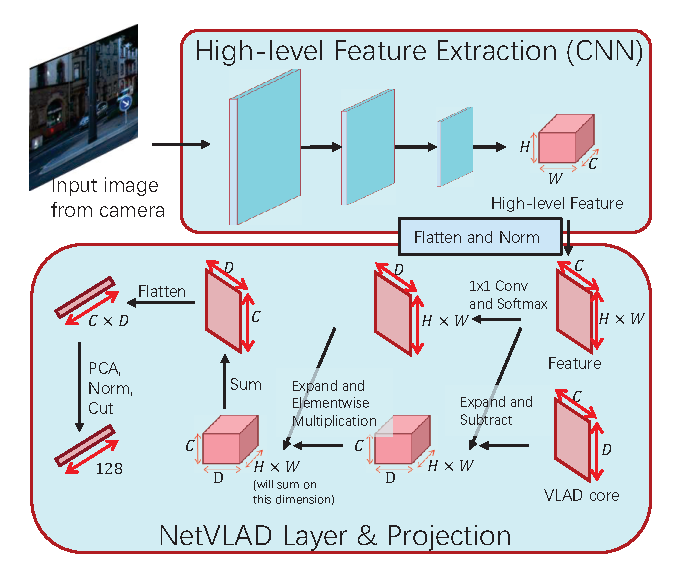
\includegraphics[width=0.85\linewidth]{fig/NetVLAD.eps}
    \caption{Process of NetVLAD.}
    \label{fig:NetVLAD}
\end{figure}